\documentclass{article}
\usepackage{amsmath, amssymb, amsfonts, bm, mathtools, graphics}
\usepackage[tmargin=1in,bmargin=1in,lmargin=1.25in,rmargin=1.25in]{geometry}
\usepackage[utf8]{inputenc}
\renewcommand{\theequation}{\thesection.\arabic{equation}}
\newcommand{\qed}{\tag*{$\square$}}
\graphicspath{ {/home/frost/Documents/College/PHYS 5630/assignments/n_sphere/plots/} }
\begin{document}
    
Class: PHYS 5630

Instructor: Bob Hirosky

Name: Quang Cap

Date: 8/27/2023

\begin{center}
    \fbox{\fbox{\parbox{35mm}{\centering First Class Project}}}
\end{center}

\[
    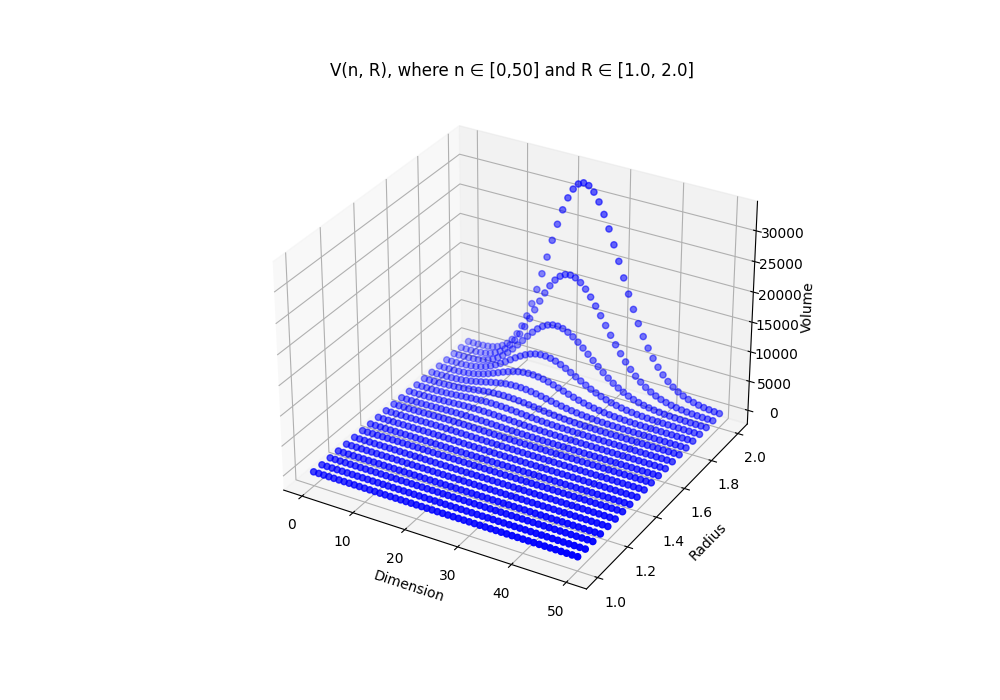
\includegraphics[width=15cm, height=12cm]{volumes}
\]

\begin{align*}
    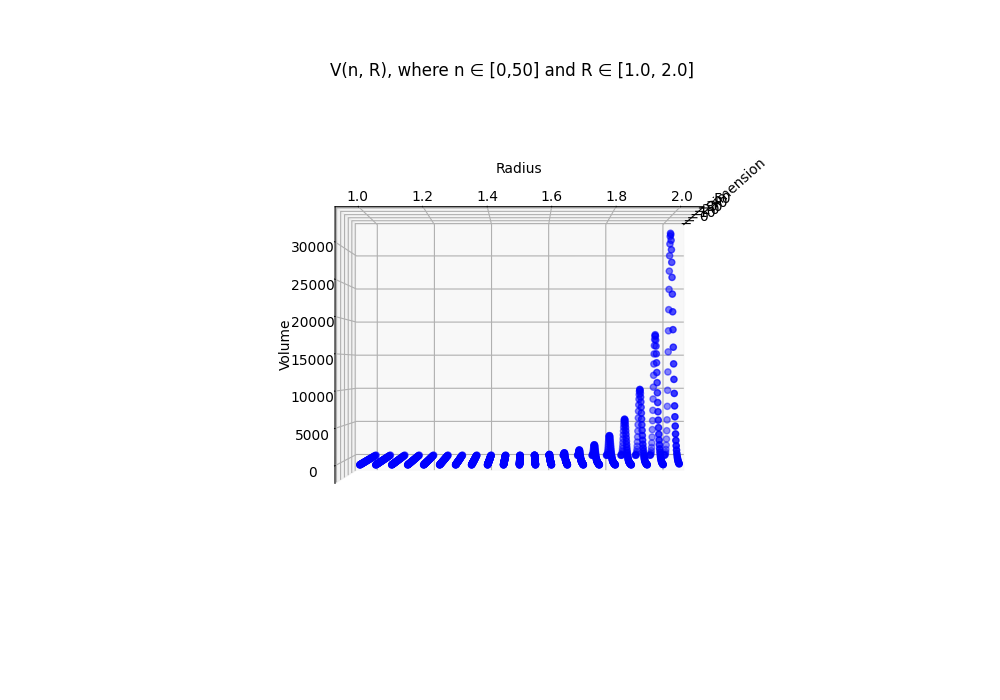
\includegraphics[width=15cm, height=12cm]{volumes_radii} \\
    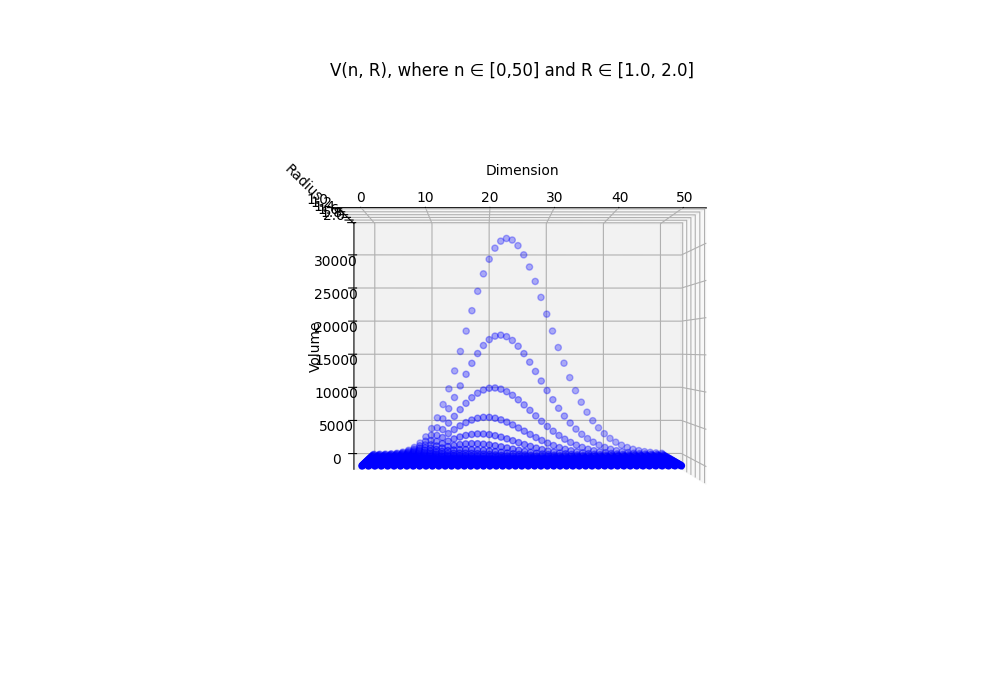
\includegraphics[width=15cm, height=12cm]{volumes_dimensions}
\end{align*}

\begin{align*}
    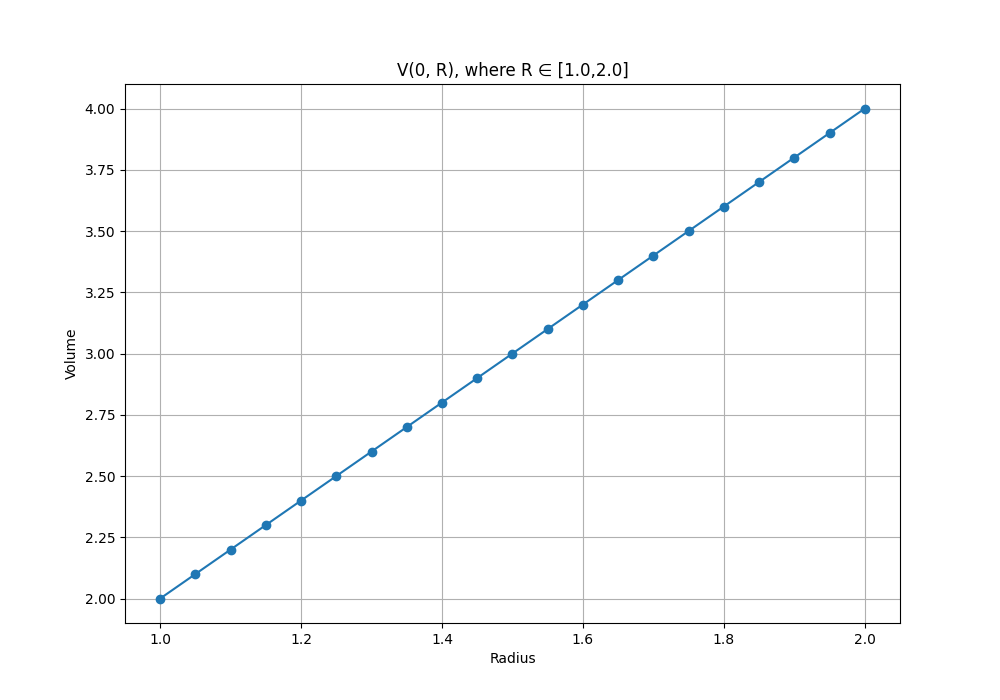
\includegraphics[width=15cm, height=12cm]{volumes_dim0_r.png} \\
    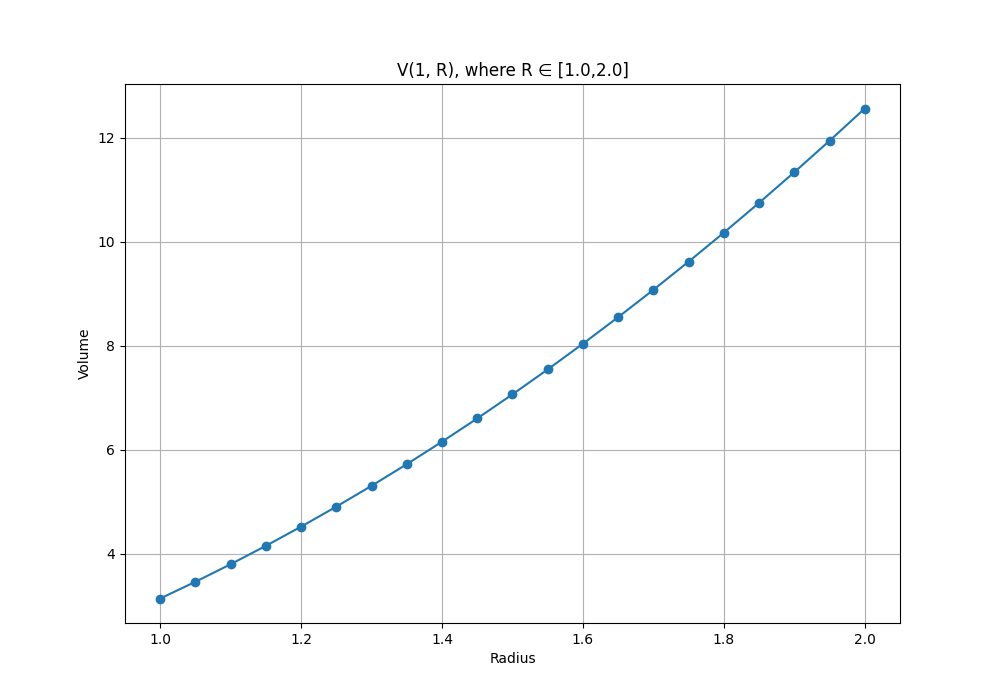
\includegraphics[width=15cm, height=12cm]{volumes_dim1_r.png}
\end{align*}

\begin{align*}
    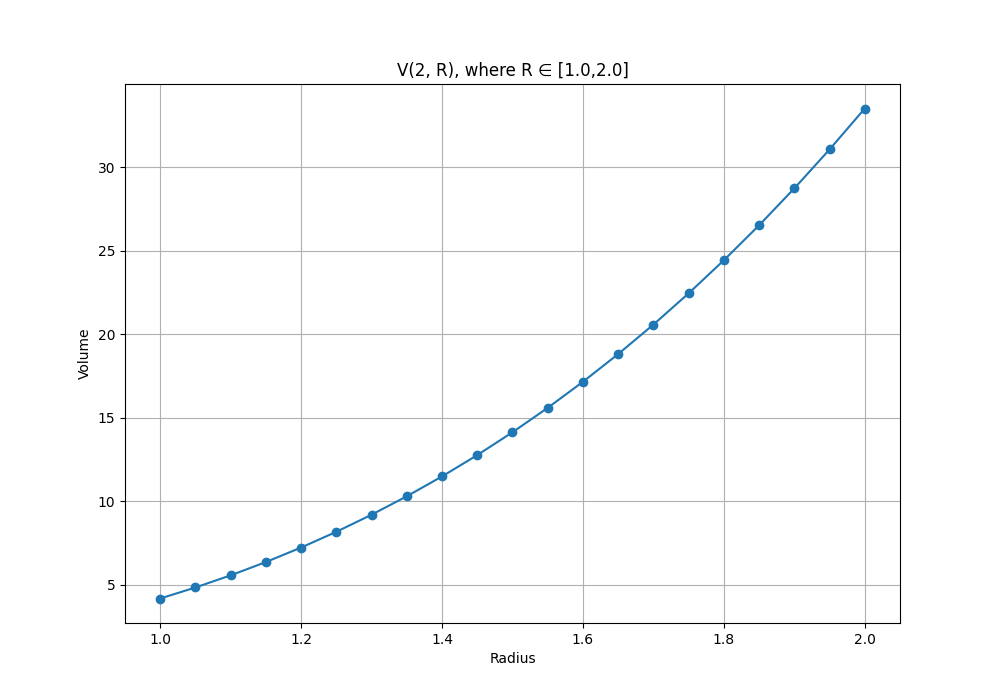
\includegraphics[width=15cm, height=10cm]{volumes_dim2_r.png} \\
    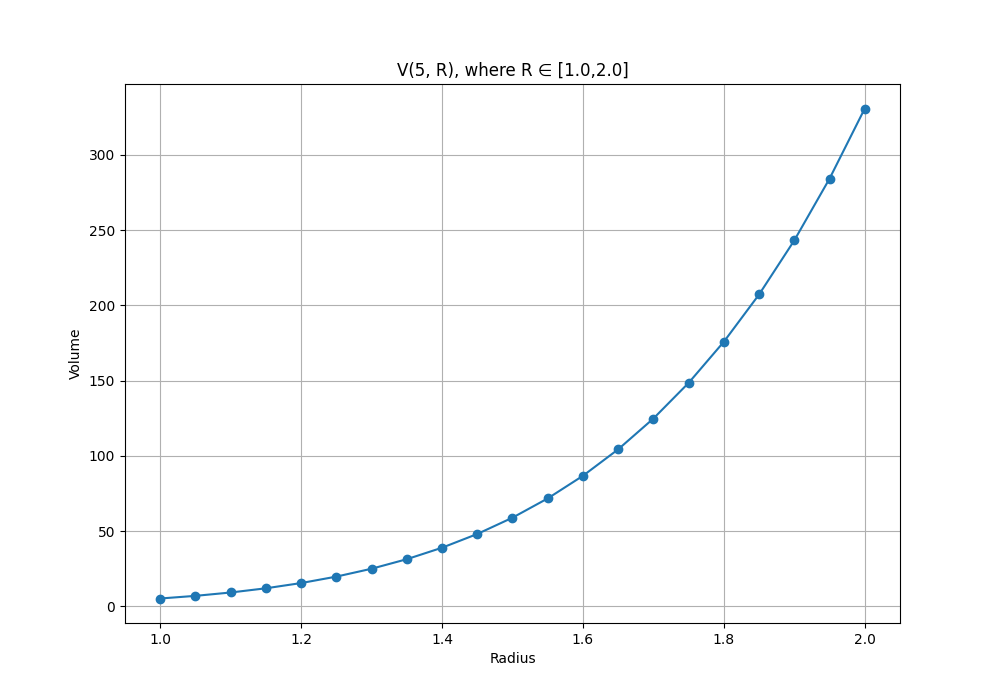
\includegraphics[width=15cm, height=10cm]{volumes_dim5_r.png}
\end{align*}

\begin{align*}
    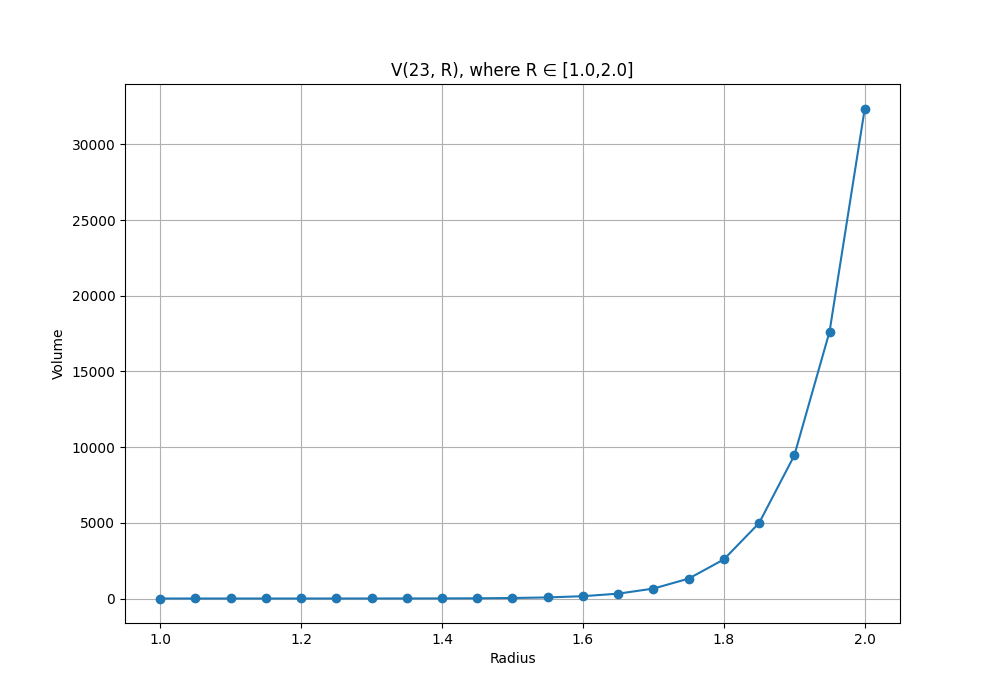
\includegraphics[width=15cm, height=10cm]{volumes_dim23_r.png} \\
    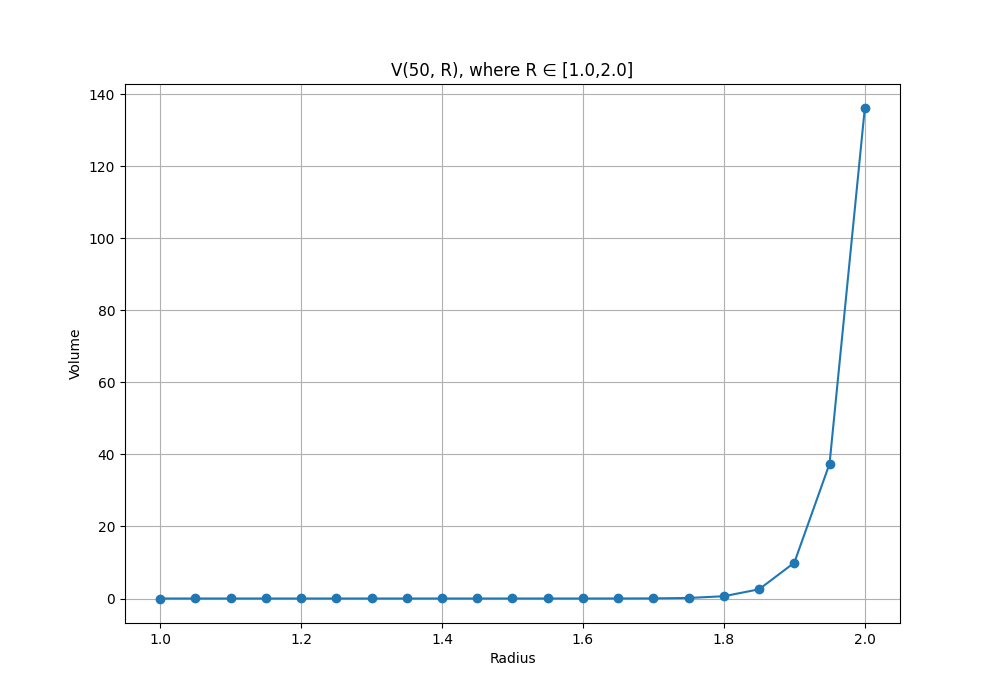
\includegraphics[width=15cm, height=10cm]{volumes_dim50_r.png}
\end{align*}

\begin{align*}
    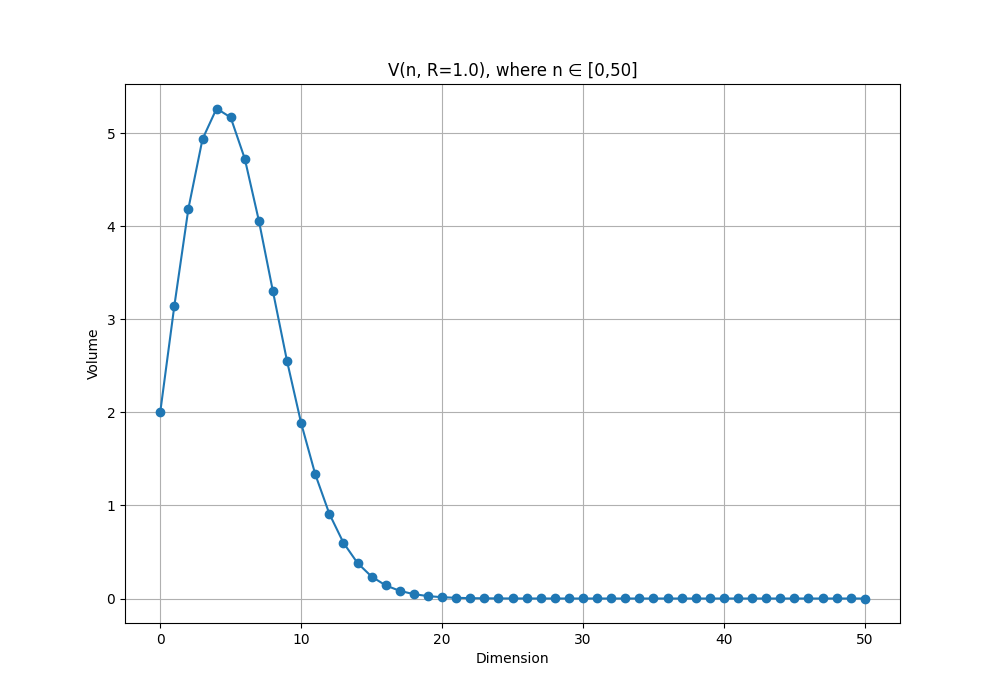
\includegraphics[width=15cm, height=10cm]{volumes_dims_r1_0.png} \\
    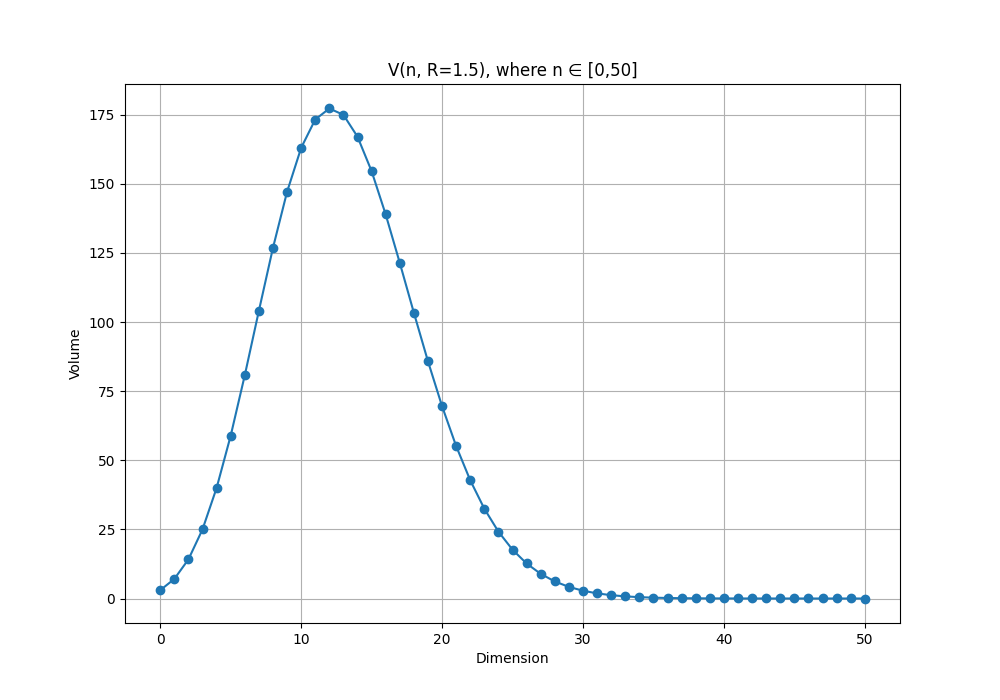
\includegraphics[width=15cm, height=10cm]{volumes_dims_r1_5.png}
\end{align*}

\[
    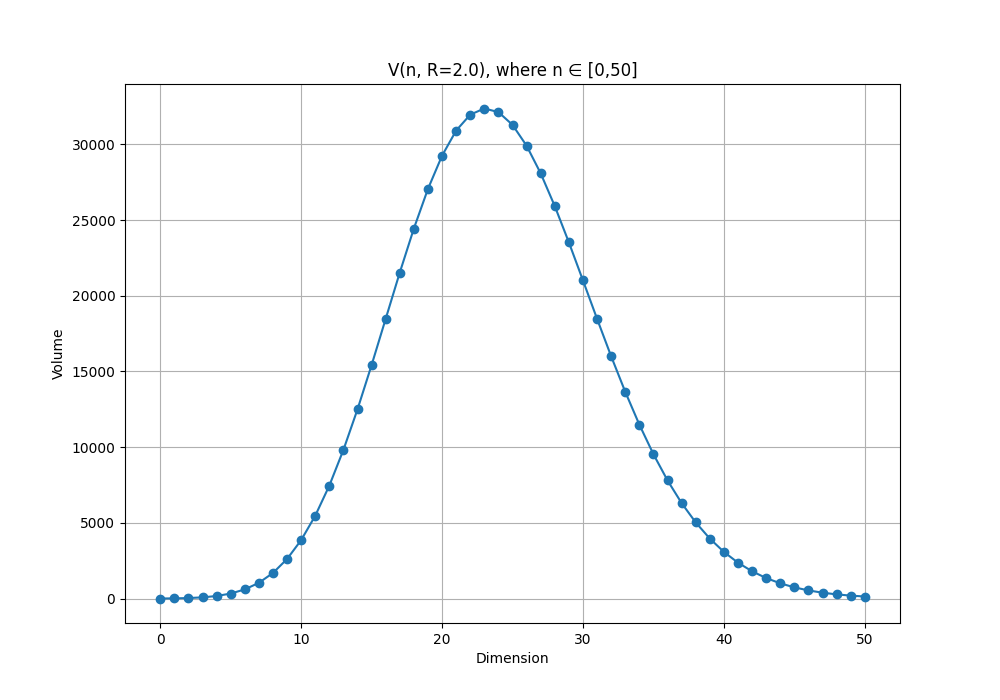
\includegraphics[width=15cm, height=10cm]{volumes_dims_r2_0.png}
\]

\end{document}